\documentclass[titlepage,landscape]{seminar}
\usepackage{url}
\usepackage{graphicx}
\usepackage[pdftex]{color}
\usepackage{hyperref}
\usepackage{epstopdf}
\usepackage{slides}

\begin{document}

\myslide{
\begin{center}
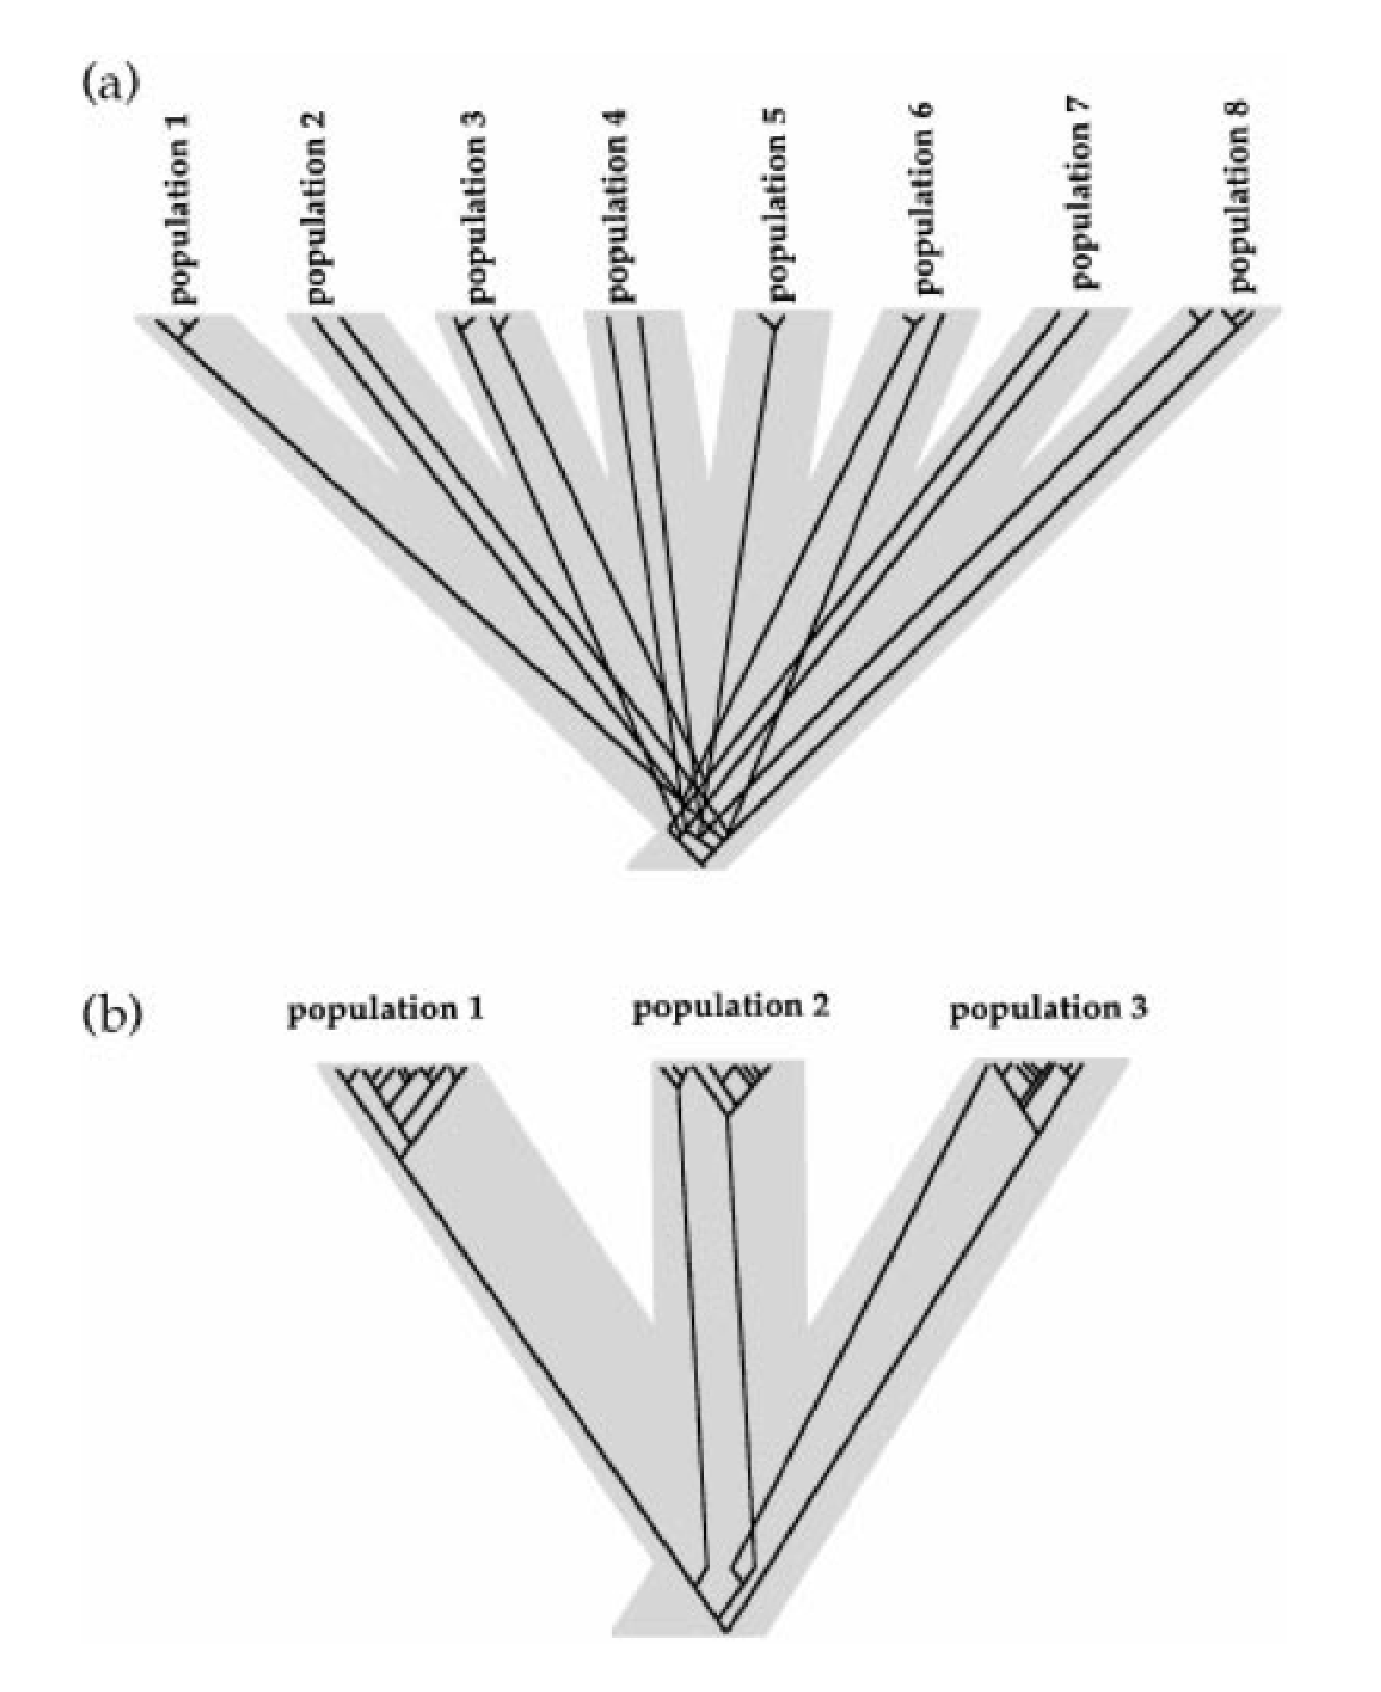
\includegraphics[height=\textheight]{divergence-hypotheses.eps}
\end{center}
}

\myslide{
\[
P(t|n, N_e) = \left(\frac{n(n-1)}{4N_e}\right)\left(1-
  \frac{n(n-1)}{4N_e}\right)^{t-1} \quad . \label{eq:coalescent-single}
\]
}

\myslide{
\begin{itemize}

\item Coalescent event
\[
P(\mbox{no coalescent}|n, N_e, K) = \left(1-\frac{n(n-1)}{4N_e}\right)^K
\]

\vfill

\end{itemize}
}

\myslide{
\begin{itemize}

\item no coalescent event
\[
P(\mbox{no coalescent}|n, N_e, K) = \left(1-\frac{n(n-1)}{4N_e}\right)^K
\]
\vfil
\item no migration event
\[
P(\mbox{no migration}|m, K) = (1-m)^{nK} 
\]
\vfill
\end{itemize}
}

\myslide{
\begin{itemize}

\item no coalescent event
\[
P(\mbox{no coalescent}|n, N_e, K) = \left(1-\frac{n(n-1)}{4N_e}\right)^K
\]
\vfil
\item no migration event
\[
P(\mbox{no migration}|m, K) = (1-m)^{nK} 
\]
\vfill
\item event: either migration or coalescent
{\small
\[
P(\mbox{event}|n, m, N_e, K) = 1 - P(\mbox{no coalescent}|n, N_e,
K)P(\mbox{no migration}|m, K) \quad .\label{eq:event}
\]
}
\end{itemize}
}

\myslide{
{\small
\[
P(\mbox{event at }t|n, m, N_e, K) = P(\mbox{event}|n, m, N_e,
K)\left(1 - P(\mbox{event}|n, m, N_e, K)\right)^{t-1}
\]
}
\vfil
\begin{eqnarray*}
P(\mbox{coalescent}) &=& \frac{1-\left(1-\frac{n(n-1)}{4N_e}\right)^K}%
{1-\left(1-\frac{n(n-1)}{4N_e}\right)^K + 1 - (1-m)^{nK}} \\
&\approx& \frac{\frac{Kn(n-1)}{4N_e}}{\frac{Kn(n-1)}{4N_e} + Knm} \\
&=& \frac{\frac{(n-1)}{4N_e}}{\frac{(n-1)}{4N_e} + m}
\end{eqnarray*}
\vfil
\[
P(\mbox{migration}) = 1 - P(\mbox{coalescent})
\]
}

\myslide{
\begin{center}
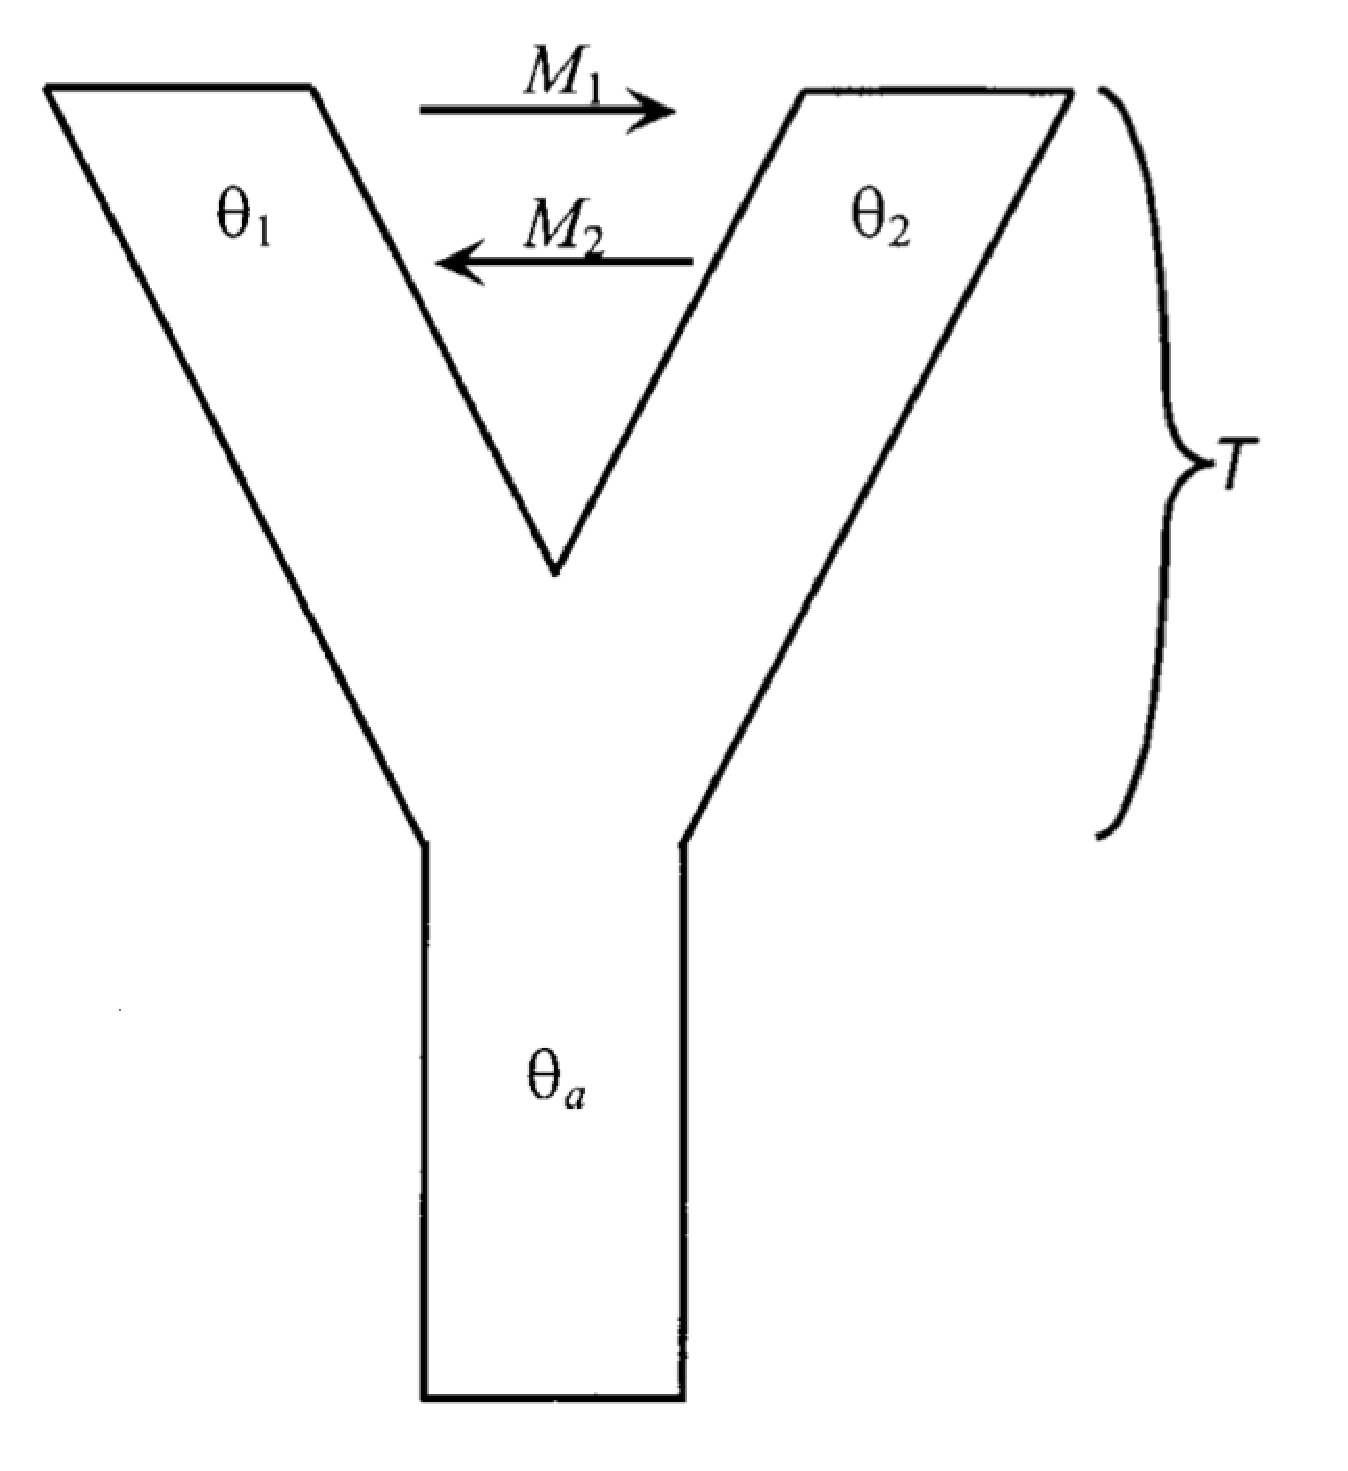
\includegraphics[width=0.65\textwidth]{nielsen-wakeley.eps}
\end{center}
}

\myslide{
\begin{center}
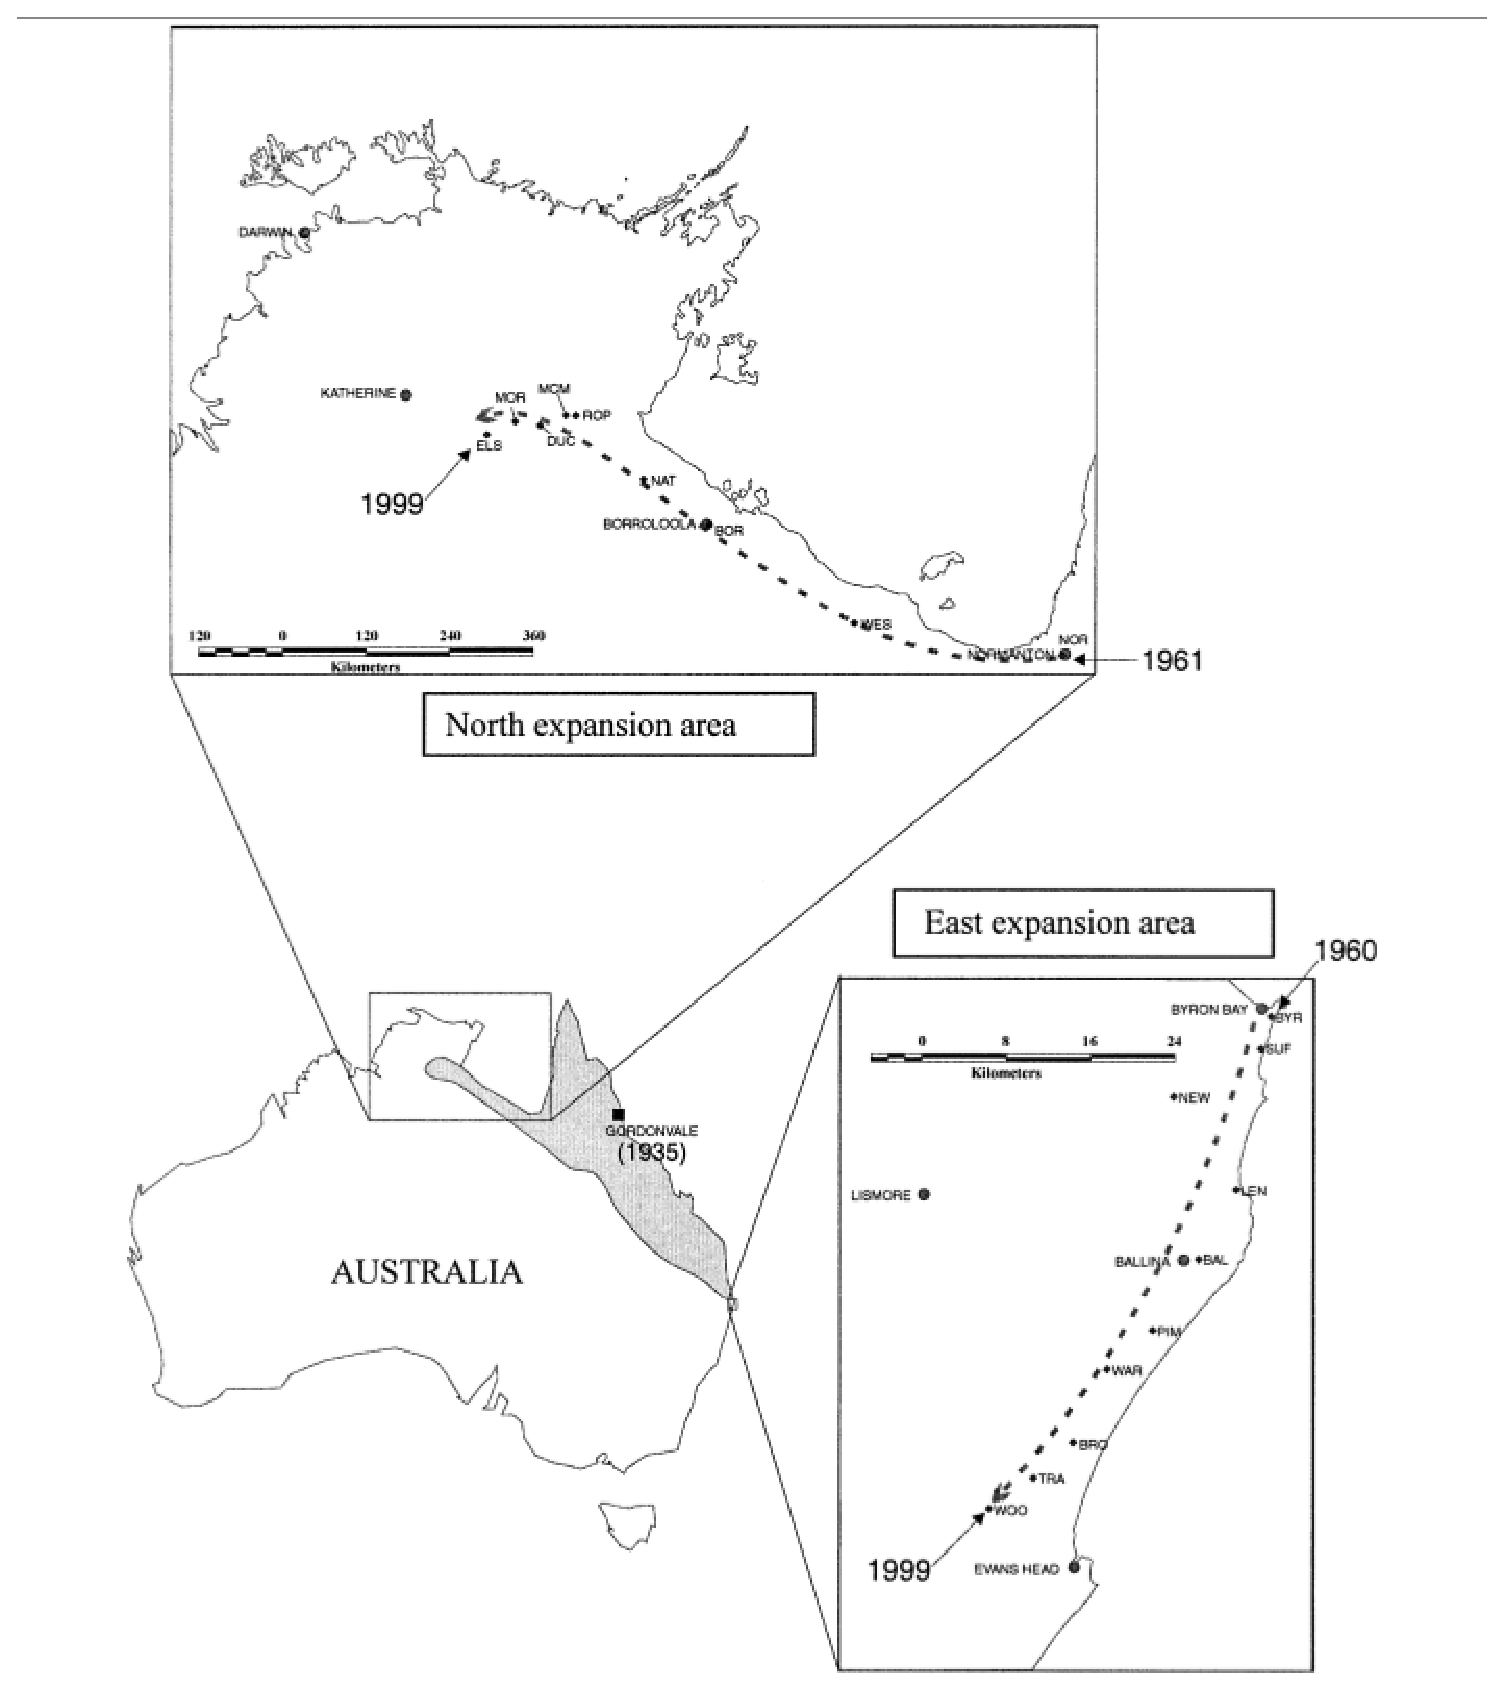
\includegraphics[width=0.65\textwidth]{cane-toad-expansion.eps}
\end{center}
}

\myslide{
\begin{center}
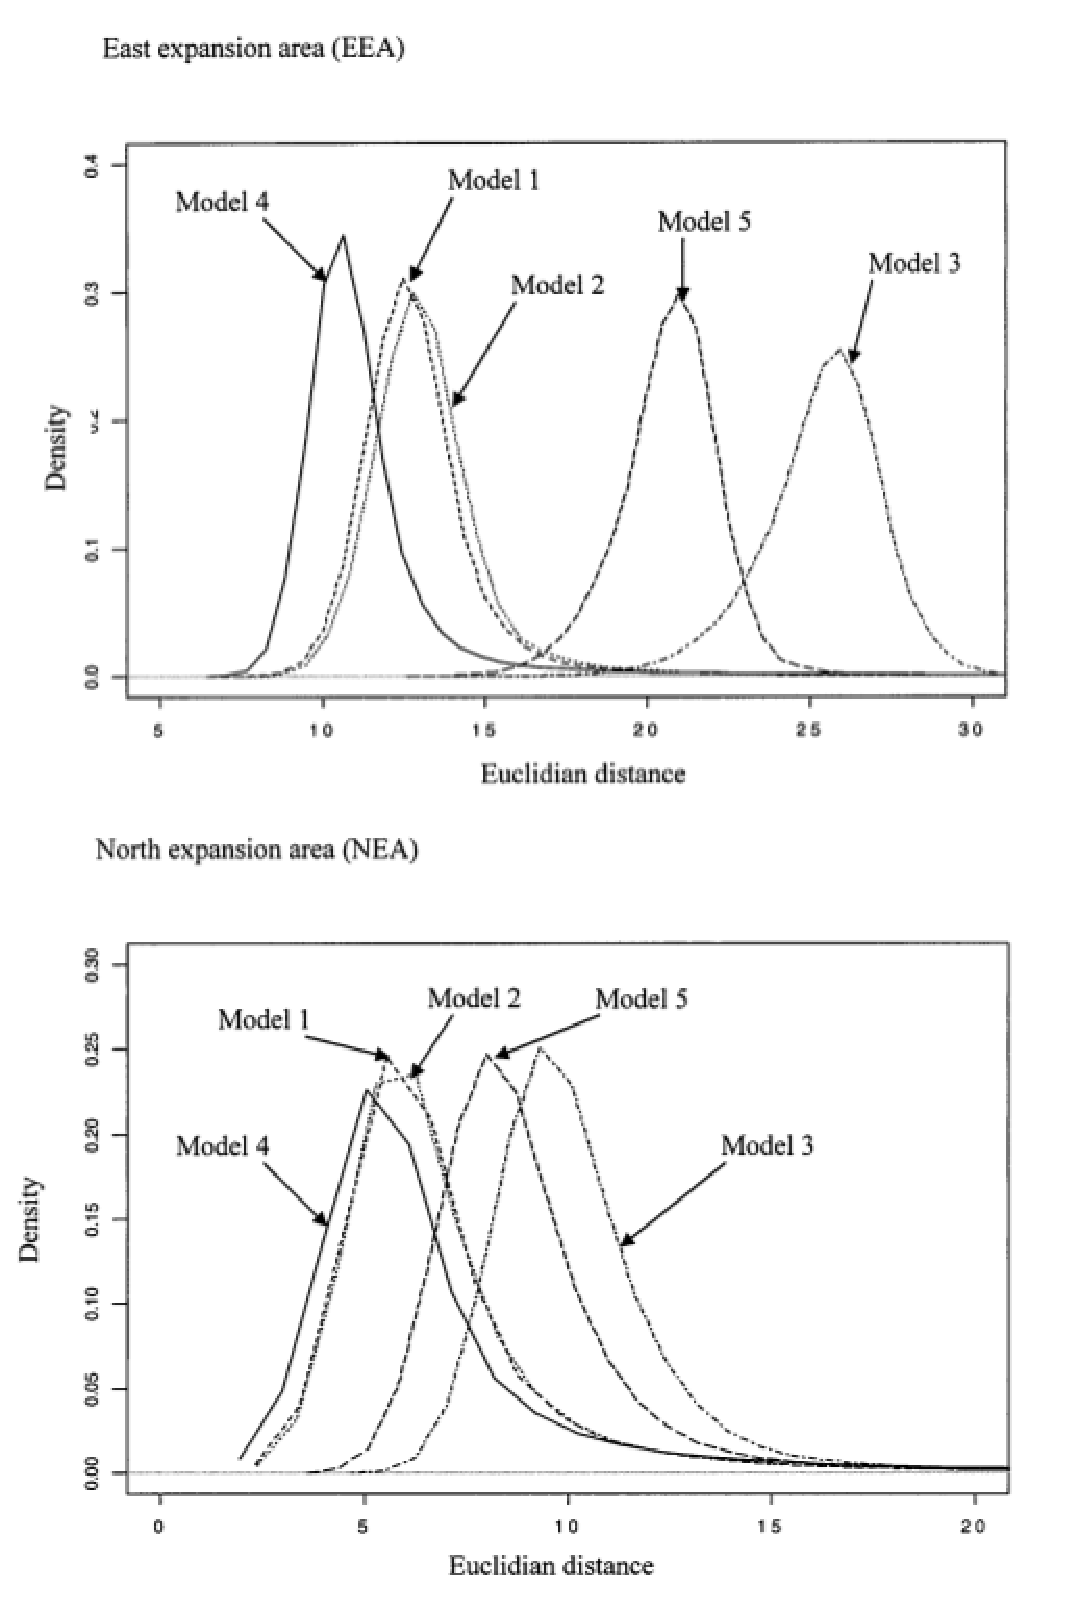
\includegraphics[height=\textheight]{cane-toad-models.eps}
\end{center}
}

\myslide{
\begin{itemize}

\item $N_{e_s}$: the effective population size when the population is
  stable.

\item $N_{e_f}$: the effective population size when a new population
  is founded.

\item $F_R$: the founding ratio, $N_{e_s}/N_{e_f}$.

\item $m$: the migration rate.

\item $N_{e_s}m$: the effective number of migrants per generation.

\end{itemize}
}

\myslide{
\begin{center}
\begin{tabular}{ccr}
\hline\hline
Parameter & area & mean (5\%, 90\%) \\
\hline
$N_{e_s}$ & east & 744 (205, 1442) \\
         & north & 1685 (526, 2838) \\
$N_{e_f}$ & east & 78 (48, 118) \\
         & north & 311 (182, 448) \\
$F_R$    & east & 10.7 (2.4, 23.8) \\
         & north & 5.9 (1.6, 11.8) \\
$m$      & east & 0.014 ($6.0 \times 10^{-6}$, 0.064) \\
         & north & 0.117 ($1.4 \times 10^{-4}$, 0.664) \\
$N_{e_s}m$ & east & 4.7 (0.005, 19.9) \\
          & north & 188 (0.023, 883) \\
\hline
\end{tabular}
\end{center}
}


\end{document}


